\documentclass[border={2pt 2pt 2pt 2pt}]{standalone}
\usepackage{tikz}
\usetikzlibrary{calc}
\begin{document}

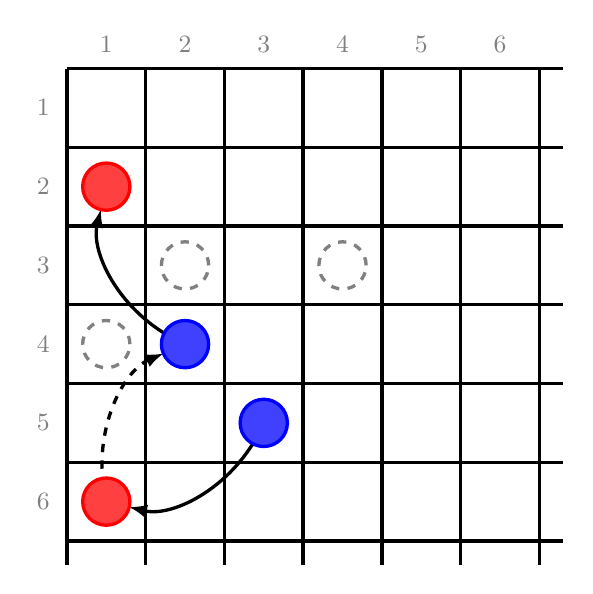
\begin{tikzpicture}[very thick]
\draw (0,-0.3) grid (6.3,6);
\draw[black,shorten >=0.3cm,dashed,-latex] (0.5,0.5) to [bend left=40] (1.5,2.5);
\draw[black,shorten >=0.3cm,-latex] (2.5,1.5) to [bend left=40] (0.5,0.5);
\draw[black,shorten >=0.3cm,-latex] (1.5,2.5) to [bend left=40] (0.5,4.5);
\draw[blue,very thick,fill=blue!75] (2.5,1.5) circle [radius=.3];
\draw[red,very thick,fill=red!75] (0.5,0.5) circle [radius=.3];
\draw[blue,very thick,fill=blue!75] (1.5,2.5) circle [radius=.3];
\draw[red,very thick,fill=red!75] (0.5,4.5) circle [radius=.3];
\draw[gray,dashed,very thick] (0.5,2.5) circle [radius=.3];
\draw[gray,dashed,very thick] (1.5,3.5) circle [radius=.3];
\draw[gray,dashed,very thick] (3.5,3.5) circle [radius=.3];
\foreach \x in {1,...,6} {
  \node[gray] at (\x-0.5,6.3) {\small\x};
  \node[gray] at (-0.3,6.5-\x) {\small\x};
}
\end{tikzpicture}
\end{document}
